\section{Evaluation}
\label{sec:eval}

\begin{figure}[h]
  \makebox[\textwidth][c]{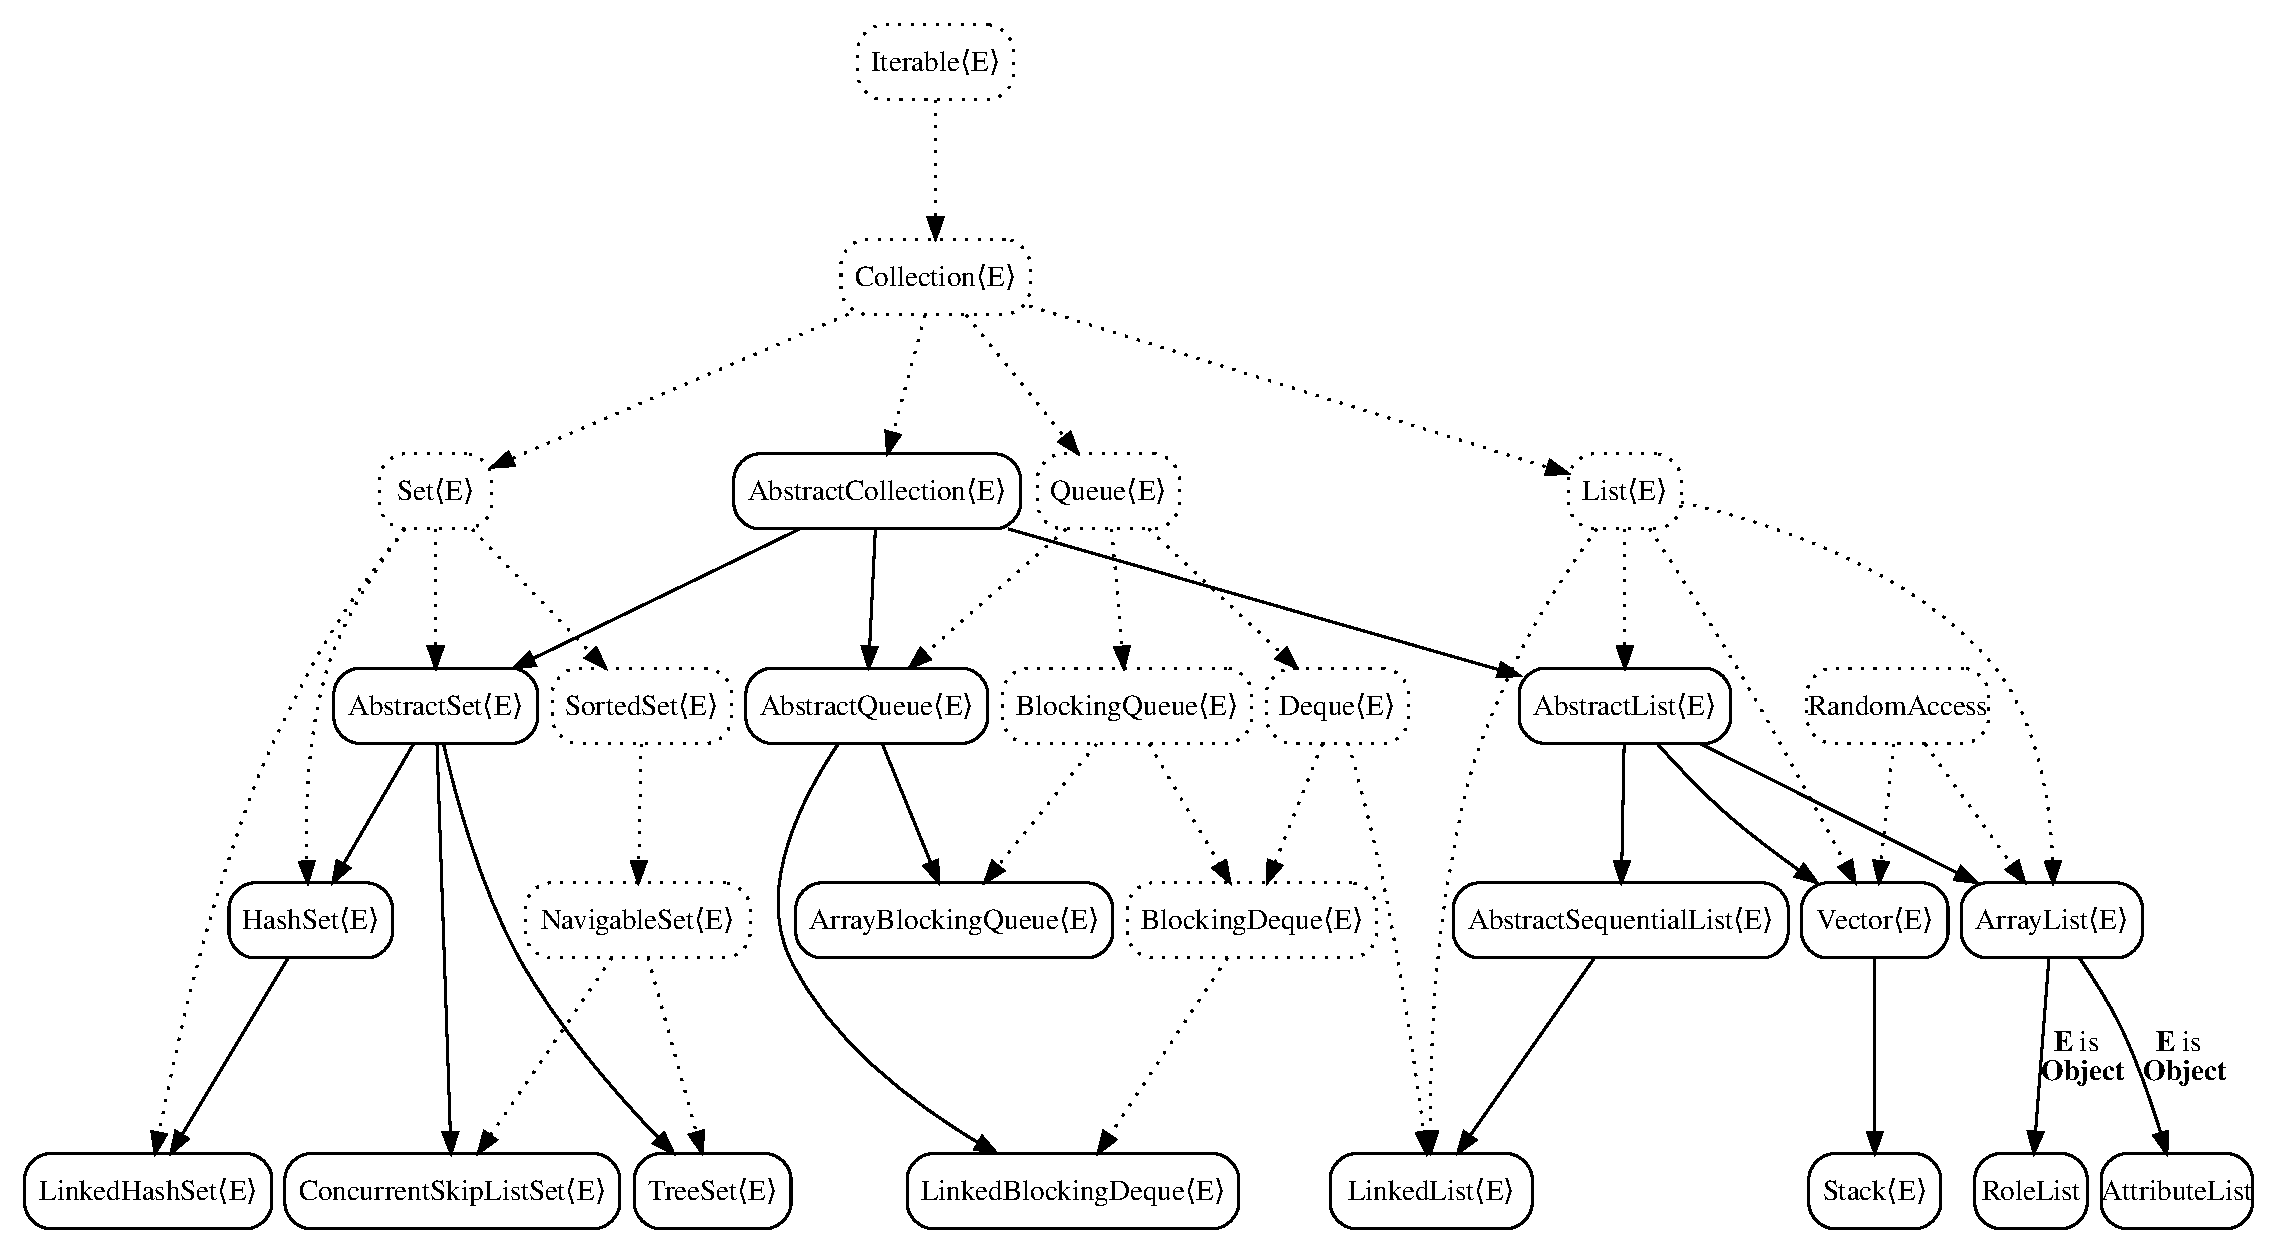
\includegraphics[width=1.3\textwidth]{class_graph.eps}}
  \caption{Evaluation class table: a subset of \textsc{Java} collection classes}
  \label{fig:class-graph}
\end{figure}

\begin{comment}
    On pic.~\ref{fig:class-graph} class \textbf{AbstractCollection} extends class \textbf{Object}. Also classes \textbf{ArrayList}, \textbf{Vector}, \textbf{LinkedList}, \textbf{HashSet}, \textbf{TreeSet}, \textbf{ConcurrentSkipListSet} and \textbf{LinkedHashSet} implements interfaces \textbf{Cloneable} and \textbf{Serializable}. Classes \textbf{BlockingQueue} and \textbf{LinkedBlockingDeque} implements interface \textbf{Serializable} only.
\end{comment}

To perform the evaluation of the solver we came up with we prepared a sample class table using a subset of standard \textsc{Java} collection classes and interfaces. The
inheritance graph for this subset is shown in Fig.~\ref{fig:class-graph}; the nodes with sold border correspond to classes, with dashed border~--- to interfaces.

Our first attempt discovered the fact that the solver was unsound~--- it established the subtyping relation for two arbitrary types. This finding constitutes a drastic
contradiction with the theory which predicts that the solver has to be correct by construction. The careful analysis, however, discovered that functional
vefifier was unsound as well! The reason was very simple: let us have two arbitrary types $A$ and $B$. To establish, for example, that $A \precprec B$, take a
type variable $\alpha^B_A$ with upper bound $B$ and lower bound $A$. Then, by definition

\[
A\precprec \alpha^B_A \wedge \alpha^B_A\precprec B \Rightarrow A\precprec B
\]

In the JLS there were no explicit requirement for lower/upper bounds of type variables to respect the subtyping relation, thus this requirement was not
encoded in the verifier.

Another finding of the evaluation was that, contrary to the expectation, the direct supertyping relation is actually reflexive (in full accordance with the JLS).

\begin{figure}[h]
    \begin{tabular}{c|c|c|c|c}
        \multirow{2}{*}{Test} & \multicolumn{2}{c|}{JGS} & \multicolumn{2}{c}{Simplified JGS} \\
        \cline{2-5}
         & Time & Answers & Time & Answers \\
         \hline
         
         ? $\precprec$ AbstractList\textlangle Object\textrangle 
         & 1.152
         & 8 / 8
         & 0.238
         & 8 / 8
         \\ \hline
         RoleList $\precprec$ ? 
         & 0.472
         & 38 / 21
         & 0.332
         & 22 / 11
         \\ \hline
         ? $\precprec$ Iterable\textlangle Object\textrangle 
         & $>$300
         & -
         & 1.912
         & 58 / 26
         \\ \hline
         ? $\precprec$ RandomAccess $\land$
         & $>$300
         & -
         & 1.326
         & 8 / 5
         \\
         ? $\precprec$ AbstractCollection\textlangle Object\textrangle 
         &&&&\\ \hline
        LinkedList\textlangle Object\textrangle $\,\precprec$ ? $\land$
        & 24.278
        & 95 / 10
        & 3.620
        & 69 / 6
        \\
        TreeSet\textlangle Object\textrangle $\,\precprec$ ?
        &&&&
    \end{tabular}
    \caption{The results of evaluation for some queries}
    \label{fig:eva}
\end{figure}

After we added explicit subtyping constraint for the bounds of type variables, we could, indeed, obtain all correct subtyping results
    for queries we took for evaluation. The results are shown in Fig.~\ref{fig:eva}.

    We encountered a few other issues. First, in the presence of capture conversion the solver works very slow and can not always
    provide answers in a reasonable time even for very simple queries (see column JGS). However, capture conversion makes the
    solver return wildcard types which are not instantiable (can not be used as types of concrete data values). In the
    scenario of usage we are aimed at such types are meaningless. Thus we evaluated a simplified version of the solver with
    capture conversion switched off (see Simplified JGS column).    
    
    Another issue is that the solver tends to return duplicating answers. In the columns ``Answers'' the numerator gives the number of
    returned answers while denominator~--- the total number of correct pairwise distinct solutions.

    We can conclude that, first, our approach discovers the incompleteness in specifications and, second, that the simplified version
    with capture conversion switched off shows a promising performance results.
    
    
    \begin{comment}
    \newpage

    \begin{itemize}
        \item Query: RoleList $\twoheadleftarrow$ ?
        \begin{itemize}
            \item Some answer examples:
            \begin{itemize}
                \item AbstractList\textlangle Object\textrangle
                \item AttributeList
                \item LinkedList\textlangle Object\textrangle
            \end{itemize}
            \item JGS
            \begin{itemize}
                \item Requested answers amount: 8
                \item Unique answers amount: 8
                \item Time measurement: 1.13, 1.18, 1.16, 1.15, 1.14
                \item Time average: 1.152
            \end{itemize}
            \item Simplified JGS
            \begin{itemize}
                \item Requested answers amount: all (was 8 answers)
                \item Unique answers amount: 8
                \item Time measurement: 0.23, 0.25, 0.23, 0.24, 0.24
                \item Time average: 0.238
            \end{itemize}
        \end{itemize}
        \newpage
        \item Query: RoleList $\twoheadleftarrow$ ?
        \begin{itemize}
            \item Some answer examples:
            \begin{itemize}
                \item Object
                \item RandomAccess
                \item AbstactCollection\textlangle Object\textrangle
                \item AbstactCollection\textlangle ? Extends Object\textrangle \\ (missing for the simplified JGS)
                \item AbstactCollection\textlangle ? Super Object\textrangle \\ (missing for the simplified JGS)
            \end{itemize}
            \item JGS
            \begin{itemize}
                \item Requested answers amount: all (was 38 answers)
                \item Unique answers amount: 21
                \item Time measurement: 0.41, 0.50, 0.50, 0.46, 0.49
                \item Time average: 0.472
            \end{itemize}
            \item Simplified JGS
            \begin{itemize}
                \item Requested answers amount: all (was 22 answers)
                \item Unique answers amount: 11
                \item Time measurement: 0.31, 0.36, 0.34, 0.31, 0.34
                \item Time average: 0.332
            \end{itemize}
        \end{itemize}
        \newpage
        \item Query: ? $\twoheadleftarrow$ Iterable\textlangle Object\textrangle
         \begin{itemize}
            \item Some answer examples:
            \begin{itemize}
                \item List\textlangle Object\textrangle
                \item AttributeList
                \item LinkedHashSet\textlangle Object\textrangle
                \item Vector\textlangle Object\textrangle
                \item LinkedBlockingDeque\textlangle Object\textrangle
            \end{itemize}
            \item JGS
            \begin{itemize}
                \item Requested answers amount: 58
                \item Time measurement: more than 300 seconds
            \end{itemize}
            \item Simplified JGS
            \begin{itemize}
                \item Requested answers amount: all (was 58 answers)
                \item Unique answers amount: 26
                \item Time measurement: 1.88, 1.94, 1.94, 1.89, 1.91
                \item Time average: 1.912
            \end{itemize}
        \end{itemize}
        \newpage
        \item Query: ? $\twoheadleftarrow$ RandomAccess $\land$ ? $\twoheadleftarrow$ AbstractCollection\textlangle Object\textrangle
         \begin{itemize}
            \item All unique answers:
            \begin{itemize}
                \item ArrayList\textlangle Object\textrangle
                \item Vector\textlangle Object\textrangle
                \item AttributeList
                \item RoleList
                \item Stack\textlangle Object\textrangle
            \end{itemize}
            \item JGS
            \begin{itemize}
                \item Requested answers amount: 8
                \item Time measurement: more than 300 seconds
            \end{itemize}
            \item Simplified JGS
            \begin{itemize}
                \item Requested answers amount: all (was 8 answers)
                \item Unique answers amount: 5
                \item Time measurement: 1.32, 1.32, 1.34, 1.33, 1.32
                \item Time average: 1.326
            \end{itemize}
        \end{itemize}
        \newpage
        \item Query: ? LinkedList\textlangle Object\textrangle $\,\twoheadleftarrow$ ? \\ $\land$  TreeSet\textlangle Object\textrangle $\,\twoheadleftarrow$ ?AbstractCollection\textlangle Object\textrangle
         \begin{itemize}
            \item Some answer examples:
            \begin{itemize}
                \item AbstactCollection\textlangle Object\textrangle
                \item Cloneable
                \item Serializable
                \item Iterable\textlangle Object\textrangle
                \item Collection\textlangle Object\textrangle
                \item Object
            \end{itemize}
            \item JGS
            \begin{itemize}
                \item Requested answers amount: all (was 95 answers)
                \item Unique answers amount: 10
                \item Time measurement: 24.09, 25.01, 24.47, 24.04, 23.78
                \item Time average: 24.278
            \end{itemize}
            \item Simplified JGS
            \begin{itemize}
                \item Requested answers amount: all (was 69 answers)
                \item Unique answers amount: 6
                \item Time measurement: 3.61, 3.67, 3.59, 3.64, 3.59
                \item Time average: 3.620
            \end{itemize}
        \end{itemize}
    \end{itemize}   
\end{comment}
